\documentclass[10pt]{article}
\usepackage{itcep, stmaryrd, tikz, pgflibraryplotmarks, multicol, pgfplots}
\usepackage[margin=1in, nohead, pdftex]{geometry}

\topmargin -0.2in
\pagestyle{empty}
\singlespacing
\let\oldhat\hat
\renewcommand{\vec}[1]{\mathbf{#1}}
\renewcommand{\hat}[1]{\oldhat{\mathbf{#1}}}

\definecolor{light-gray}{gray}{0.95}
\newcommand{\code}[1]{\colorbox{light-gray}{\texttt{#1}}}

\newcommand{\headerclass}{Machine Learning Camp}
\newcommand{\headersection}{Day 2: Introduction to Classification}
\newcommand{\headertitle}{Put to the Test}

\def\C{\mathbb{C}}
\def\R{\mathbb{R}}
\parindent 0ex
\begin{document}
%==================================================================================================================================================
\headerclass\xspace \hspace{\stretch{1}} \headersection\\
\begin{center}{ \large \textbf{\headertitle} }\end{center}
%==================================================================================================================================================

\begin{center}
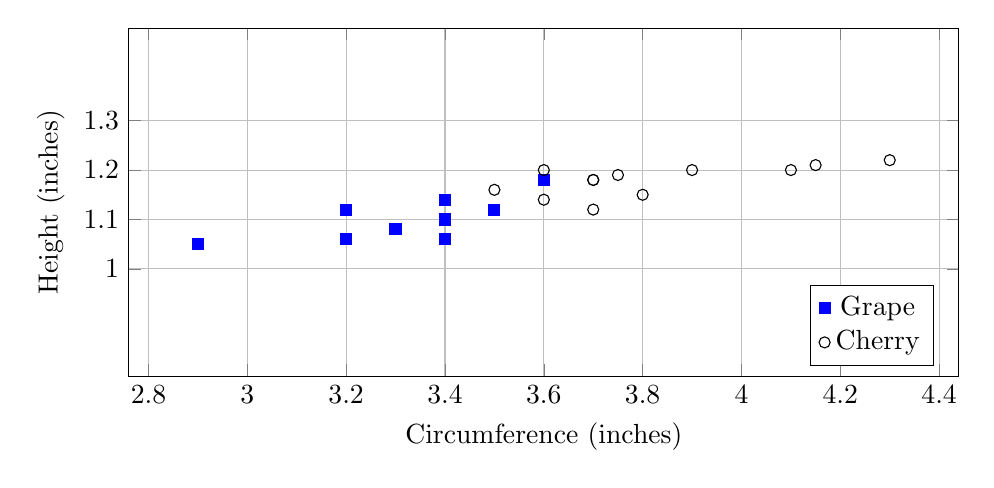
\begin{tikzpicture}
\begin{axis}[grid=both,
	legend pos=south east,
    xlabel= {Circumference (inches)},
    ylabel= {Height (inches)},
    width = \textwidth,
    height = 6cm,
    ytick={1,1.1,1.2,1.3},
    axis equal
  ]
    \addplot[
        scatter,only marks,scatter src=explicit symbolic,
        scatter/classes={
            a={mark=square*,blue},
            b={mark=o,draw=black,fill=black}
        }
    ]
    table[x=x,y=y,meta=label]{
        y    x    label
        1.18 3.7 b
        1.06 3.2 a
        1.08 3.3 a
        1.06 3.4 a
        1.05 2.9 a
        1.12 3.5 a
        1.14 3.4 a
        1.18 3.6 a
        1.18 3.7 b
        1.16 3.5 b
        1.14 3.6 b
        1.12 3.7 b
        1.19 3.75 b
        1.20 3.9 b
        1.20 3.6 b
        1.22 4.3 b
        1.20 4.1 b
        1.21 4.15 b
        1.15 3.8 b
        1.1 3.4 a
        1.12 3.2 a

    };
    \legend{Grape, Cherry}
\end{axis}
\end{tikzpicture}
\end{center}

Intuitively, we saw that the $3$-nearest neighbor algorithm seemed to be better at classifying grapes and cherries than the $1$-nearest neighbor algorithm. In order to verify this, we'll divide our given data into a \emph{training set} and a \emph{testing set}.\\

The \emph{training set} will be used for classification. So, we'll figure out the cherry and grape regions based only on the data from the training set. It's called the ``training set'' because it's used to \emph{train} the algorithm - it's how the algorithm learns what to do!\\

The \emph{testing set} will be used to evaluate how well our classification algorithm is performing. For each data point $P$ from the testing set, we'll use $k$-nearest neighbor algorithm to predict whether $P$ is a grape or a cherry. Then, we'll check if the algorithm was correct.\\

Below, we've separated our data into a training set and a testing set. The points from the training set are plotted above, and the points from the testing set are in the table below.

\begin{center}
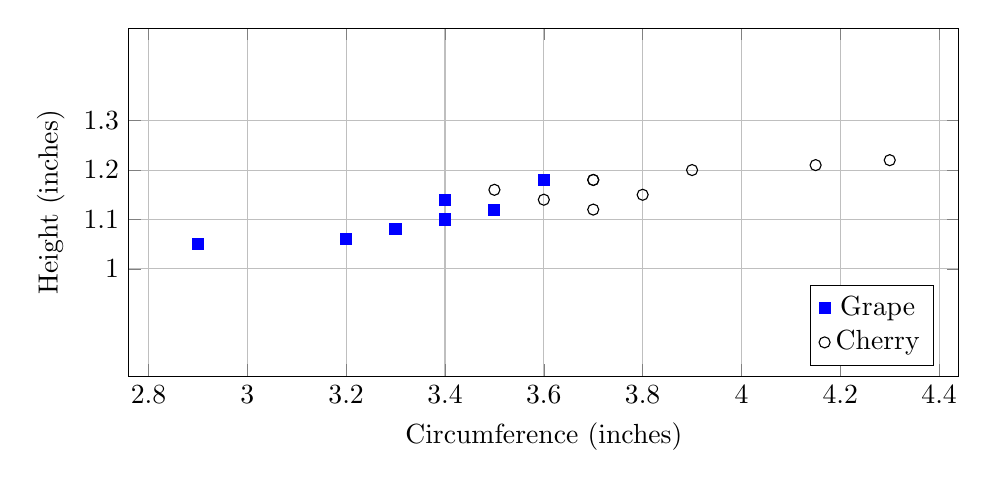
\begin{tikzpicture}
\begin{axis}[grid=both,
	legend pos=south east,
    xlabel= {Circumference (inches)},
    ylabel= {Height (inches)},
    width = \textwidth,
    height = 6cm,
    ytick={1,1.1,1.2,1.3},
    axis equal
  ]
    \addplot[
        scatter,only marks,scatter src=explicit symbolic,
        scatter/classes={
            a={mark=square*,blue},
            b={mark=o,draw=black,fill=black}
        }
    ]
    table[x=x,y=y,meta=label]{
        y    x    label
        1.18 3.7 b
        1.06 3.2 a
        1.08 3.3 a
        1.05 2.9 a
        1.12 3.5 a
        1.14 3.4 a
        1.18 3.6 a
        1.18 3.7 b
        1.16 3.5 b
        1.14 3.6 b
        1.12 3.7 b
        1.20 3.9 b
        1.22 4.3 b
        1.21 4.15 b
        1.15 3.8 b
        1.1 3.4 a


    };
    \legend{Grape, Cherry}
\end{axis}
\end{tikzpicture}
\end{center}

\begin{center}
\begin{tabular}{|p{3.5cm}|p{3.5cm}|p{2cm}|}
\hline
Circumference (inches) & Height (inches) & Fruit\\
\hline
 3.2 & 1.12 & Grape\\\hline
 4.1 & 1.2 & Cherry\\\hline
 3.4 & 1.06 & Grape\\\hline
 3.75 & 1.19 & Cherry\\\hline
 3.6 & 1.20 & Cherry\\
 
\hline
\end{tabular}
\end{center}

\newpage

In order to compare $1$-nearest neighbor classification and $3$-nearest neighbor classification, we'll measure how accurately each algorithm is able to classify the testing set.

Let's start with $1$-nearest neighbor classification. Using the training set below, shade in the Cherry region for the $1$-nearest neighbor algorithm.

\begin{center}
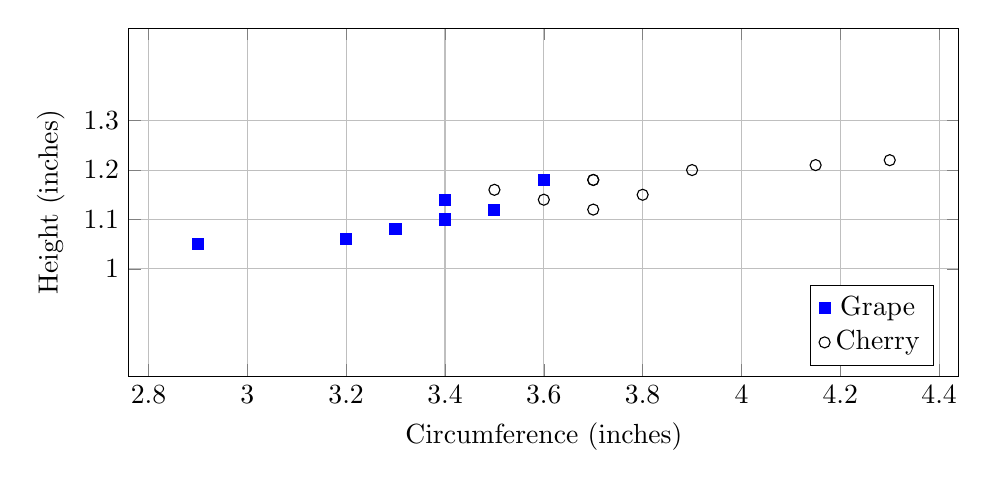
\begin{tikzpicture}
\begin{axis}[grid=both,
	legend pos=south east,
    xlabel= {Circumference (inches)},
    ylabel= {Height (inches)},
    width = \textwidth,
    height = 6cm,
    ytick={1,1.1,1.2,1.3},
    axis equal
  ]
    \addplot[
        scatter,only marks,scatter src=explicit symbolic,
        scatter/classes={
            a={mark=square*,blue},
            b={mark=o,draw=black,fill=black}
        }
    ]
    table[x=x,y=y,meta=label]{
        y    x    label
        1.18 3.7 b
        1.06 3.2 a
        1.08 3.3 a
        1.05 2.9 a
        1.12 3.5 a
        1.14 3.4 a
        1.18 3.6 a
        1.18 3.7 b
        1.16 3.5 b
        1.14 3.6 b
        1.12 3.7 b
        1.20 3.9 b
        1.22 4.3 b
        1.21 4.15 b
        1.15 3.8 b
        1.1 3.4 a


    };
    \legend{Grape, Cherry}
\end{axis}
\end{tikzpicture}
\end{center}

For each point in the testing set, plot it on the graph above, and use the $1$-nearest neighbor algorithm to predict if it's a grape or a cherry. Then check if your prediction is correct, filling in ``Yes'' or ``No''.

\begin{center}
\begin{tabular}{|p{3.5cm}|p{3cm}|p{2.5cm}|p{2cm}|p{2cm}|}
\hline
Circumference (inches) & Height (inches) & Predicted Fruit & Actual Fruit & Correct?\\
\hline
 3.2 & 1.12 & \phantom{\large A} & Grape &\\\hline
 4.1 & 1.2 &\phantom{\large A} & Cherry & \\\hline
 3.4 & 1.06 & \phantom{\large A} & Grape & \\\hline
 3.75 & 1.19 & \phantom{\large A} & Cherry & \\\hline
 3.6 & 1.20 & \phantom{\large A} & Cherry & \\\hline
\end{tabular}
\end{center}

What percent of your predictions were correct?
\vfill

We can also organize our results into a \emph{confusion matrix}, by counting how many times each combination of predicted fruit and actual fruit occurs.
\[
\left(
\text{
\begin{tabular}{p{1.8in}|p{1.8in}}
number of cherries that were predicted to be cherries & number of cherries that were predicted to be grapes\\\hline
number of grapes that were predicted to be cherries & number of grapes that were predicted to be grapes
\end{tabular}
}
\right)
\]
What is the confusion matrix for your results?
\vfill

\newpage

Next, let's evaluate the precision of $3$-nearest neighbor classification. Using the training set below, shade in the Cherry region for the $3$-nearest neighbor algorithm.

\begin{center}
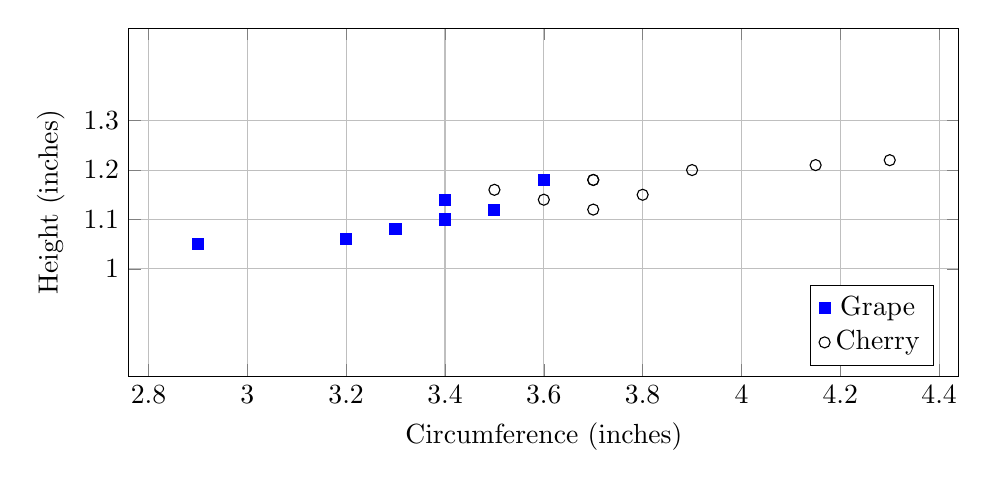
\begin{tikzpicture}
\begin{axis}[grid=both,
	legend pos=south east,
    xlabel= {Circumference (inches)},
    ylabel= {Height (inches)},
    width = \textwidth,
    height = 6cm,
    ytick={1,1.1,1.2,1.3},
    axis equal
  ]
    \addplot[
        scatter,only marks,scatter src=explicit symbolic,
        scatter/classes={
            a={mark=square*,blue},
            b={mark=o,draw=black,fill=black}
        }
    ]
    table[x=x,y=y,meta=label]{
        y    x    label
        1.18 3.7 b
        1.06 3.2 a
        1.08 3.3 a
        1.05 2.9 a
        1.12 3.5 a
        1.14 3.4 a
        1.18 3.6 a
        1.18 3.7 b
        1.16 3.5 b
        1.14 3.6 b
        1.12 3.7 b
        1.20 3.9 b
        1.22 4.3 b
        1.21 4.15 b
        1.15 3.8 b
        1.1 3.4 a


    };
    \legend{Grape, Cherry}
\end{axis}
\end{tikzpicture}
\end{center}

For each point in the testing set, plot it on the graph above, and use the $3$-nearest neighbor algorithm to predict if it's a grape or a cherry. Then check if your prediction is correct, filling in ``Yes'' or ``No''.

\begin{center}
\begin{tabular}{|p{3.5cm}|p{3cm}|p{2.5cm}|p{2cm}|p{2cm}|}
\hline
Circumference (inches) & Height (inches) & Predicted Fruit & Actual Fruit & Correct?\\
\hline
 3.2 & 1.12 & \phantom{\large A} & Grape &\\\hline
 4.1 & 1.2 &\phantom{\large A} & Cherry & \\\hline
 3.4 & 1.06 & \phantom{\large A} & Grape & \\\hline
 3.75 & 1.19 & \phantom{\large A} & Cherry & \\\hline
 3.6 & 1.20 & \phantom{\large A} & Cherry & \\\hline
\end{tabular}
\end{center}

What percent of your predictions were correct?
\vfill

What is the confusion matrix for your results?
\vfill

Which was more accurate, classification using the $1$-nearest neighbor algorithm or classification using the $3$-nearest neighbor algorithm?
\vfill

How does the choice of the split between training and testing sets affect the algorithm? What are some ``bad'' ways to split the data?
\vfill

\end{document}
